% !TEX encoding = UTF-8
% !TEX TS-program = pdflatex
% !TEX root = ../tesi.tex

%**************************************************************
\chapter{Valutazione}
\label{cap:resoconto-stage}
%**************************************************************

%**************************************************************
\section{Soddisfacimento degli obiettivi}
Il progetto di stage ha avuto una durata di 316 ore, oltre la durata minima ma in linea con quella massima di 320 ore.\\
Negli ultimi due giorni di stage ho preparato, e successivamente esposto, una presentazione del lavoro svolto, durante il periodo di stage, al mio tutor, Giuseppe Pavan, al \textit{team leader} e sviluppatore \textit{senior}, Riccardo Cardin, e al CTO di \textit{\azienda}, Guido Ronchetti \footnote{Guido Ronchetti: Linkedin= \link{https://www.linkedin.com/in/guido-ronchetti-285637a/}}. Grazie a questa presentazione ho potuto ricevere un \textit{feedback} del lavoro svolto, riassumere al \textit{team} dell'azienda che mi ha ospitato la mia analisi tecnologica e le idee su questi tipi di base di dati ed, infine, fare esperienza nella preparazione di un discorso tecnico da esporre a persone con esperienza decennale.\\
Attraverso i documenti consegnati, il prototipo e la presentazione da me svolti, l'azienda ha potuto acquisire le informazioni necessarie per valutare il passaggio a questo tipo di tecnologia. Chiaramente questo mio progetto non può sostituire una vera analisi di fattibilità con i relativi costi per lo studio di nuove tecnologie e conseguenze tecniche dovute al cambiamento. Il mio prodotto potrà servire, però, all'azienda per determinare se vale la pena svolgere questo tipo di attività e individuare nuove funzionalità dovute al cambiamento. Tutto questo risparmiando sia risorse sia tempo, che a volte in un azienda possono essere limitate.\\
Gli obiettivi obbligatori, come descritto nella \hyperlink{sec:pianodl}{sezione 2.1.3}, si concentravano sull'analisi delle varie tecnologie di basi di dati a grafo e sulla progettazione e realizzazione di un prototipo che esemplifichi le capacità di queste. Sono stati soddisfatti completamente risparmiando un numero significativo di ore lavoro. Con le ore rimaste mi sono concentrato nel migliorare il prototipo, aggiungendo funzionalità interessanti, e nel soddisfare un requisito opzionale, cioè la preparazione di una presentazione interna del lavoro svolto.
\newpage
\section{Conoscenze acquisite}
Le conoscenze che, grazie a questa esperienza di stage, ho acquisito o semplicemente ampliato sono le seguenti.
\subsubsection{Base di dati a grafo}
Durante questo progetto ho potuto avvicinarmi ai \textit{database} organizzati a grafo, tecnologia che ignoravo prima di questa esperienza.\\
Inizialmente, questa tecnologia mi è sembrata simile alle basi di dati relazionali. Informandomi e testandola con il mio prototipo, però, ho compreso le sue potenzialità. Quasi tutti i vantaggi sono dati dalla possibilità di attraversare i nodi in tempo costante e non dipendente dalla grandezza del \textit{database}, questo non avviene in quelli relazionali a causa delle operazioni di \gls{JOIN}.\\
Mi ritengo soddisfatto di aver acquisito delle conoscenze in questa materia grazie all'evoluzione che sta avendo in questo ultimo periodo, rispetto alle altre tipologie di base di dati.
\begin{figure}[h!]
	\centering
	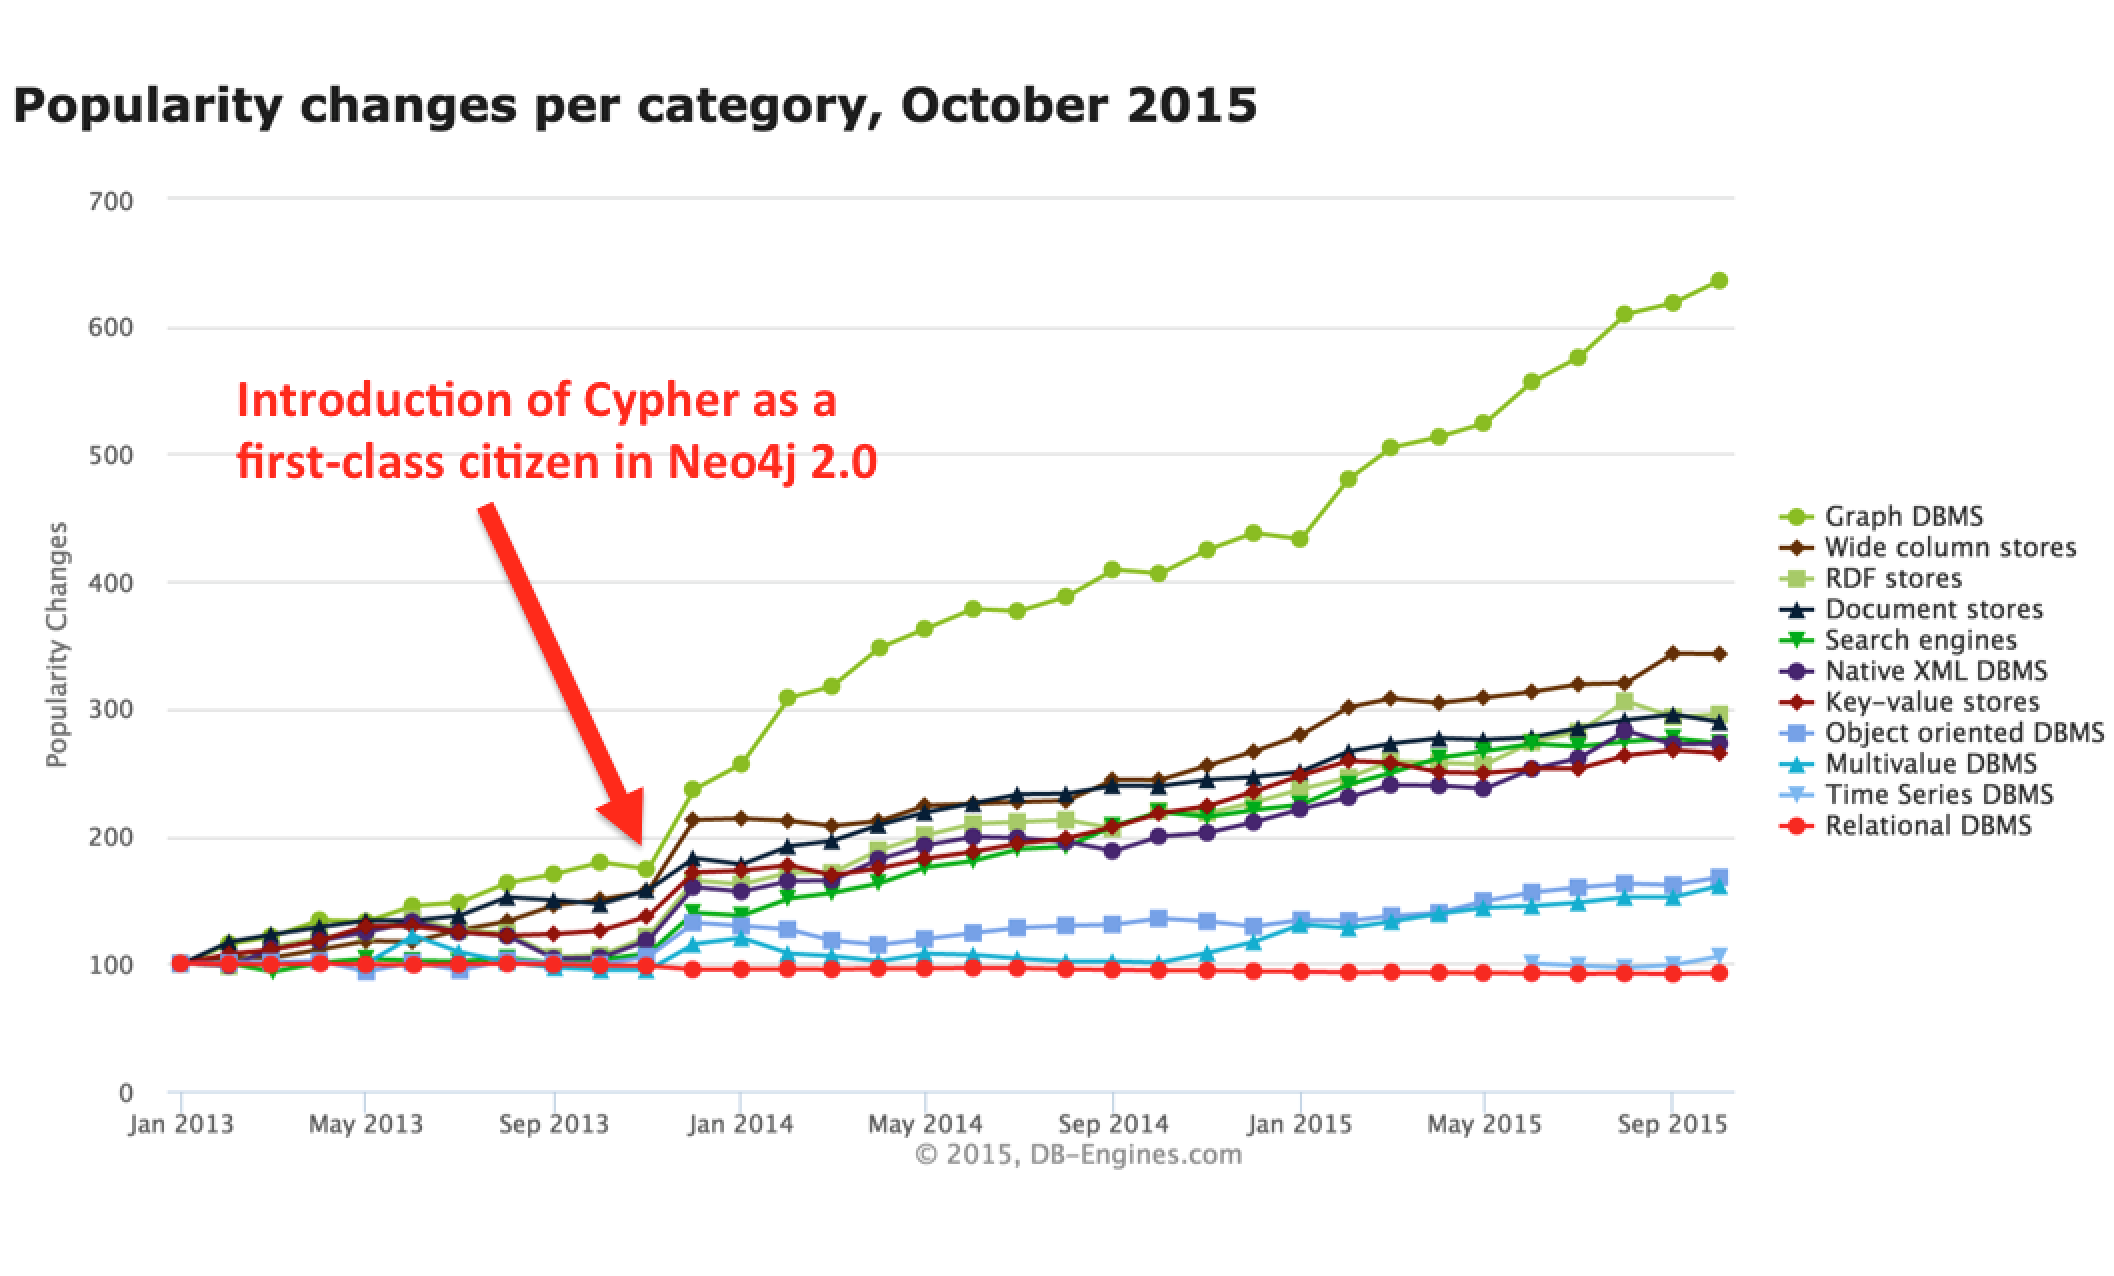
\includegraphics[scale=0.4]{immagini/graphchange.png}
	\label{fig:figura 2.2}
	\caption{\textit{Evoluzioni delle base di dati a grafo rispetto alle altre tipologie \link{https://goo.gl/SfV3vZ}}}
\end{figure}
\newpage
\subsubsection{Capacità di condurre una analisi tecnologica}
Attraverso questa esperienza ho potuto acquisire capacità di condurre una analisi tecnologica strutturata. Ho imparato ad individuare le possibili alternative, eseguire una scrematura utilizzando un confronto strutturato ed uniforme per caratteristiche ed, infine, scegliere la migliore in base al caso d'uso di riferimento. Tutto questo aiutandomi con le documentazioni ufficiali delle alternative tecnologiche e \textit{forum} di riferimento quali StackOverflow\footnote{StackOverflow: url= \link{https://stackoverflow.com/}} e Dzone\footnote{Dzone: url= \link{https://dzone.com/}}.
\subsubsection{Progettazione e realizzazione di un'applicazione Java}
Ho potuto acquisire capacità di progettare e realizzare autonomamente una applicazione Java sfruttando \textit{\gls{framework}} avanzati come Spring\footnote{Spring: url= \link{https://spring.io/}} e utilizzare, anche se superficialmente, la tecnologia Docker\footnote{Docker: url= \link{https://www.docker.com/}}.
\section{Valutazione personale}
Per quanto riguarda questa esperienza di stage mi ritengo soddisfatto del lavoro svolto, in termini di requisiti e qualità del prodotto finale, e del progetto di stage scelto. Purtroppo non ho potuto soddisfare completamente i requisiti opzionali sia per mancanza di tempo che per l'impossibilità di recuperare, o solamente analizzare, dati reali per le stringenti politiche sulla \textit{privacy} di dati sensibili.\\
Mi ritengo soddisfatto, invece, del progetto scelto perchè lo ritengo un giusto compromesso tra una analisi, che mi ha portato a svolgere una tesi con buoni contenuti, ed un progetto di sviluppo che mi ha permesso di acquisire conoscenze che sfrutterò nel mondo del lavoro.\\
Infine ritengo il progetto di stage, in un azienda esterna, l'unico modo per acquisire nozioni che durante il corso di studi sarebbe molto difficile conseguire in così poco tempo. Personalmente estenderei l'obbligo di stage a molti altri corsi di studi universitari che non lo contengono.
\section{Differenza tra università e mondo del lavoro}
Durante la mia esperienza lavorativa ho notato un \textit{gap} rispetto al percorso di studi universitario. Questa differenza si focalizza nella mancanza di conoscenza nelle tecnologie avanzate, come particolari \textit{\gls{framework}}, oppure di nuova generazione. Questa mancanza è sopperita, però, dall'insegnamento durante i corsi universitari dei concetti di base che mi hanno portato ad imparare ed adattarmi velocemente a queste nuove tecnologie. Ciò non significa che non si debba aggiorare i percorsi di studi con un programma adatto al mondo lavorativo odierno.\\ Personalmente valuterei l'aggiunta, da parte dell'università, di un insegnamento che avvicini lo studente alle basi di dati non relazionali e l'uso avanzato di Java, spiegando le nuove funzionalità introdotte con le recenti versioni di questo linguaggio.\\
Inoltre aggiungerei, ad un corso già presente, un avvicinamento ai sistemi di controllo di versione, invece di delegare totalmente allo studente l'onere di impararlo durante gli svariati progetti universitari.\\
Un'altra cosa che mi ha lasciato perplesso durante il mio percorso universitario è stata la scelta di non insegnare, nel corso di tecnologie \textit{web}, tecnologie di rilievo, anche se non definite da \textit{standard}, come HTML5\footnote{HTML5: url= \link{https://www.w3schools.com/html/html5\textunderscore intro.asp}}.\\
Al netto di questi dettagli il mio percorso di studi mi ha permesso di acquisire nozioni ed aspetti fondamentali dell'informatica che non sarei riuscito ad imparare autonomamente. Inoltre è riuscito a far si che mi appassionassi alla materia nonostante, prima dell'iscrizione all'Università di Padova, la mia conoscenza a questa fosse nulla. \\Considero molto importante la presenza dei progetti universitari: mi hanno insegnato a lavorare in un \textit{team}, mantenuto alta la voglia di migliorarmi e permesso di aggiungere un'esperienza dimostrabile al mio \textit{curriculum}, oltre a tutte le nozioni tecniche che ho appreso.

